155. Прямоугольный лист бумаги разделили на четыре части, одна из которых --- квадрат. Периметры серых прямоугольников равны 34 см и 22 см. Найдите: а) периметр; б) площадь листа бумаги.
\begin{center}
\begin{figure}[ht!]
\center{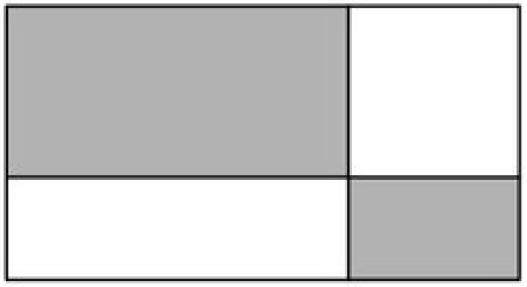
\includegraphics[scale=0.35]{37.png}}
\end{figure}
\end{center}
ewpage
oindent
